\begin{heading}[label=chap:headings]{chapter}
  \tpTitle{coco-headings.sty}
\end{heading}
\index{coco-headings|textbf}

This module handles the processing and typesetting of heading
complexes. It's top-level Namespace is \texttt{heading}.

\begin{heading}[label=sec:hdg]{section}
  \tpTitle{User Macros}
\end{heading}

\begin{heading}[label=sec:hdg:headingenv]{subsection}
  \tpTitle{The \mytexttt{heading} Environment}
\end{heading}

In the {\LaTeX} code, headings are represented in the \textit{heading}\index[tex]{heading@\texttt{heading}*}
environment.
\begin{lstlisting}[style=tex]
\begin{heading}[<Options>]{<Level>}
  \tpTitle{<Main Title>}
\end{heading}
\end{lstlisting}
The mandatory argument of that environment specifies the name of the
heading level, in most cases this is something like \textit{part},
\textit{chapter}, \textit{subsection}, etc.. \lstinline{<Level>} may
be an arbitrary string as long as the heading environment has been
declared (see \fullref{sec:hdg:decl}).

\begin{heading}[label=sec:hdg:comp:options]{subsubsection}
  \tpTitle{Heading Options}
\end{heading}

The following options for \lstinline{heading} environments are implemented:
\begin{description}
\item[label=<label>] Label for the heading. This can be used to
  reference the heading with \LaTeX's crossref macros like
  \lstinline{\ref}, \lstinline{\pageref}, etc.
\item[notoc] This heading will create no entry in the Table of Contents.
\item[nonumber] This heading will create no heading nunmber if the
  \lstinline{numbering} Property for this level is set to
  \lstinline{auto}.
\end{description}

\begin{heading}[label=sec:hdg:comp]{subsection}
  \tpTitle{Pre-Defined Components}
\end{heading}

\begin{heading}[label=sec:hdg:comp:predef]{subsubsection}
  \tpTitle{Components}
\end{heading}

The pre-defined components of a heading are:
\begin{description}
\item[\string\tpTitle]\index[tex]{tpTitle@\texttt{\textbackslash tpTitle}} The heading's main title,
\item[\string\tpSubtitle] its subtitle\index[tex]{tpSubtitle@\texttt{\textbackslash tpSubtitle}},
\item[\string\tpAuthor] the section or chapter's author\index[tex]{tpAuthor@\texttt{\textbackslash tpAuthor}},
\item[\string\tpNumber] the counter of the heading,\index[tex]{tpNumber@\texttt{\textbackslash tpNumber}}
\item[\string\tpQuote] a quote,\index[tex]{tpQuote@\texttt{\textbackslash tpQuote}}
\item[\string\tpQuoteSource] the quote's source,\index[tex]{tpQuoteSource@\texttt{\textbackslash tpQuoteSource}}
\end{description}
The only mandatory Component of a heading is the \lstinline{Title}
component. All other components may be omitted.

\begin{heading}{subsubsection}
  \tpTitle{Extended Components}
\end{heading}

There is an extended set of predefined components when a heading level is using the property \lstinline{extended}:
\begin{description}
\item[\string\tpAbstract] an abstract\index[tex]{tpAbstract@\texttt{\textbackslash tpAbstract}}
\item[\string\tpAbstractLabel] the Title for the abstract (``Abstract'' if omitted),\index[tex]{tpAbstractTitle@\texttt{\textbackslash tpAbstractLabel}}
\item[\string\tpKeywords] a list of keywords \index[tex]{tpKeywords@\texttt{\textbackslash tpKeywords}}
\item[\string\tpKeywordsLabel] the Title of the list of keywords (``Keywords'' if omitted)\index[tex]{tpKeywordsTitle@\texttt{\textbackslash tpKeywordsLabel}}
\item[\string\tpDOI] the DOI of contribution\index[tex]{tpKeywords@\texttt{\textbackslash tpKeywords}}
\item[\string\tpDOILabel] the title of the DOI (``DOI'' if omitted)\index[tex]{tpKeywordsTitle@\texttt{\textbackslash tpKeywordsLabel}}
\end{description}


\begin{heading}[label=sec:hdg:comp:overrides]{subsubsection}
  \tpTitle{Overrides}\index{Headings!Overrides}
\end{heading}

The components \lstinline{Title}\index{Title},
\lstinline{Subtitle}\index{Subtitle},
\lstinline{Author}\index{Author}, and \lstinline{Number}\index{Number}
each have further component macros that are prefixed with
\lstinline{Run}, \lstinline{Toc}, or \lstinline{BM}
respectively. Those are used to override\index{Overrides} the
Component contents when used in the running page header or footer
(henceforth, “runnning head”), in the table of contents (hf.,
“ToC”), and in the PDF bookmarks, respectively.

They are
\begin{description}
\item[\string\tpRunTitle]\index[tex]{tpRunTitle@\texttt{\textbackslash tpRunTitle}}
\item[\string\tpRunSubtitle]\index[tex]{tpRunSubtitle@\texttt{\textbackslash tpRunSubtitle}}
\item[\string\tpRunAuthor]\index[tex]{tpRunAuthor@\texttt{\textbackslash tpRunAuthor}}
\item[\string\tpRunNumber]\index[tex]{tpRunNumber@\texttt{\textbackslash tpRunNumber}}
\end{description}
for the running head,
\begin{description}
\item[\string\tpTocTitle]\index[tex]{tpTocTitle@\texttt{\textbackslash tpTocTitle}}
\item[\string\tpTocSubtitle]\index[tex]{tpTocSubtitle@\texttt{\textbackslash tpTocSubtitle}}
\item[\string\tpTocAuthor]\index[tex]{tpTocAuthor@\texttt{\textbackslash tpTocAuthor}}
\item[\string\tpTocNumber]\index[tex]{tpTocNumber@\texttt{\textbackslash tpTocNumber}}
\end{description}
for the entries in the ToC, and
\begin{description}
\item[\string\tpBMTitle]\index[tex]{tpBMTitle@\texttt{\textbackslash tpBMTitle}}
\item[\string\tpBMSubtitle]\index[tex]{tpBMSubtitle@\texttt{\textbackslash tpBMSubtitle}}
\item[\string\tpBMAuthor]\index[tex]{tpBMAuthor@\texttt{\textbackslash tpBMAuthor}}
\item[\string\tpBMNumber]\index[tex]{tpBMNumber@\texttt{\textbackslash tpBMNumber}}
\end{description}
for the bookmarks.

One example of their usage is:
\begin{lstlisting}[style=tex]
\begin{heading}{chapter}
  \tpTitle{A Heading with some additional Text}
  \tpRunTitle{A Heading}
  \tpTocTitle{My Heading}
  \tpBMTitle{Heading}
\end{heading}
\end{lstlisting}
would print \textit{“A Heading with some additional Text”} in the
text, but \textit{“A Heading”} in the running head, \textit{“My
  Heading”} in the ToC, and \textit{“Heading”} in the PDF bookmark
list.

It is important to notice that the BM overrides are an override for
the \lstinline{Toc} macro family rather than the default,
non-prefixed, Components. That is, if the macros prefixed with
\lstinline{BM} are omitted, the final values for \lstinline{Toc}
prefixed components is used to generate the bookmarks. The
\lstinline{Toc} overrides, on the other hand, use the regular heading
Components as their fallback. Therefore, only once both \lstinline{BM}
and \lstinline{Toc} overrides for a component are omitted, the
contents of the actual heading component is used for the bookmarks.

The resulting ranking of override macros can be represented as
follows:
\begin{itemize}
\item \lstinline{\tpToc<Component>} $\gg$ \lstinline{\tp<Component>}
\item \lstinline{\tpRun<Component>} $\gg$ \lstinline{\tp<Component>}
\item \lstinline{\tpBM<Component>} $\gg$ \lstinline{\tpToc<Component>} $\gg$ \lstinline{\tp<Component>},
\end{itemize}
where $x\gg y$ means that $x$ takes priority over $y$

Note that the decision on whether or not a Component is actually
printed is made elsewhere\footnote{namely, for the
  \textit{running head} it is the pagestyles that determine what is
  printed in the foot and head of left and right hand pages; the
  appearance of the \textit{ToC} and \textit{BM} entries each are
  determined via the Property lists of the various heading levels, see
  \fullref{sec:hdg:decl}.}. The overrides only control the
\textit{content} of what is printed \textit{in case the component is
  used, at all}.

One special case is the empty override\index{Overrides!Empty}
macro. It causes the Component content to be ignored when printing the
running head or ToC, respectively. E.g.,
\begin{lstlisting}[style=tex]
\begin{heading}{chapter}
  \tpNumber{Chapter 1:}
  \tpTitle{A Heading with some additional Text}
  \tpTocNumber{1:}
  \tpTocTitle{My Heading}
  \tpRunNumber{}
  \tpRunTitle{A Heading}
\end{heading}
\end{lstlisting}
would print \textit{“Chapter 1: A Heading with some additional Text”}
in the main text body; \textit{“1: My Heading”} in the ToC, and
\textit{“A Heading”} (without number!) in the running head. Also, note
that the \textit{order} of the Components within the \texttt{heading}
environment doesn't matter.

\begin{heading}[label=sec:hdg:decl]{section}
  \tpTitle{Creating New Heading Levels}\index{Headings!Creating New}
\end{heading}

The configuration of heading environments is done via the
\lstinline{\tpDeclareHeading} command:
\begin{lstlisting}[style=tex]
\tpDeclareHeading[<parent>]{<numeric_level>}{<name>}{%
  <set_properties>
}
\end{lstlisting}
where \lstinline{<numeric_level>} is a number that corresponds the
values affected by \LaTeX's \lstinline{\tocdepth} and
\lstinline{\secnumdepth} parameteres.

\lstinline{<name>} is the unique name of the heading level. This may
be something like \textit{chapter}, \textit{subpart},
\textit{paragraph}, \textit{section}, etc.

The optional argument \lstinline{<parent>} can be used to provide the
name of the heading level from which the properties should be
inherited first before the level's own properties are evaluated.

The last argument \lstinline{<set_properties>} is a list of property
assignments, see below.


\addtocontents{toc}{\protect\newpage}
\begin{heading}[label=sec:hdg:props]{section}
  \tpTitle{Heading Properties}\index{Headings!Properties}\index{Properties!Headings}
\end{heading}

Headings are configured by property assignments using the
\lstinline{\tpSetProperty} command, see \fullref{sec:set_props}.

In this section, the properties that are available to headings via the
\lstinline{coco-heading} module are listed.

\ref{fig:headingprops} gives an overview of the pre-defined
properties used in headings environments.

\begin{tpFigure}[float-pos=h]
  \tpNumber{Fig. 1}
  \tpFig{\includegraphics{images/heading-props.pdf}}
  \tpCaption{Effect of Properties on Components in the rendering of a heading environment.}
  \tpLegend{\textcolor{spot}{red} properties are dimensions; \textcolor{mblue}{blue} properties represent format markup and its scope in the default settings; \textcolor{mpurp}{purple} properties represent arbitrary {\LaTeX} markup}
  \label{fig:headingprops}
\end{tpFigure}

\endinput

\begin{heading}[label=sec:hdg:props:undef]{subsection}
  \tpTitle{Undefinable Properties}
\end{heading}

“Undefinable Properties” are properties that are generated during the
evaluation of the heading environment and therefore cannot be set
manually in a heading's declaration.\footnote{Technically, they can,
  but those assignments would be overridden every time a heading is
  rendered.}

\describeUProp{hang-number}

This property can be used to print the content of the
\lstinline{\tpNumber} Component within an \lstinline{\hbox} of a fixed
width and moved to the left by that same amount.

How wide that “hanging indent” is, depends on the values of the
\lstinline{margin-left}, \lstinline{number-width}, and
\lstinline{indent} properties, respectively. See
\fullref{sec:hdg:indent} for more details.


\begin{heading}[label=sec:hdg:props:para]{subsection}
  \tpTitle{Paragraph Control}\index{Headings!Spaces}
\end{heading}

\describeProp{interline-para}{\lstinline{<any>}}{\lstinline{<empty>}}

When an inline heading follows another inline heading and this
parameter for the latter heading level is non-empty, then the latter
will be typeset directly after the first with only the
\texttt{interline-para-sep} property between the two.

If the value is empty (default) then the second heading will be
typeset on a new par.

\describeProp{interline-para-sep}{\lstinline{<any>}}{\texttt{\textbackslash space}}

When interline-para is empty, this will be placed between two
consecutive inline headings
\Hack{\newpage}

\describeProp{heading-par}{\lstinline{<any>}}{\textit{see below}}

is the par macro that is expanded immediately before the heading is printed.

The default value is
\begin{lstlisting}[style=tex]
\tpIfProp{interline-para}{\if@noskipsec \leavevmode \fi}{}%
\par\global\@afterindenttrue%
\end{lstlisting}

\describeProp{before-heading}{\lstinline{<any>}}{\lstinline{<empty>}}

This code is executed at the very beginning of the heading
environment. This is the place where, for instance, a
\lstinline{\cleardoublepage} would be placed.


\describeProp{after-indent}{\lstinline{<any>}}{\lstinline{<empty>}}

If non-empty, this property causes the paragraph after the heading to
be indented by \lstinline{\parindent}.


\begin{heading}[label=sec:hdg:props:format]{subsection}
  \tpTitle{Formatting Headings}\index{Headings!Format}\index{Format!Headings}
\end{heading}

\describeProp{title-format}{\lstinline{<any>}}{\texttt{\string\bfseries}}

The format of the main title. It corresponds to the 6th argument of
\LaTeX's \lstinline{\@startsection} macro.

This property is applied to the \lstinline{\tpNumber} Component (if
non-empty) as well.

\describeProp{subtitle-format}{\lstinline{<any>}}{\texttt{\string\normalfont}}

The format of the \lstinline{\tpSubtitle} Component of the heading, if it exists.

\describeProp{author-format}{\lstinline{<any>}}{\texttt{\string\normalfont}}

The format of the \lstinline{\tpAuthor} Component of the heading, if it exists.

\describeProp{quote-format}{\lstinline{<any>}}{\texttt{\string\raggedleft}}

The format of the \lstinline{\tpQuote} Component of the heading, if it exists. It
also applies to the \lstinline{\tpQuoteSource} component

\describeProp{quote-source-format}{\lstinline{<any>}}{\texttt{<empty>}}

The format of the quote Component of the heading, if it exists.\Hack{\newpage}

\describeProp{heading-block}{\lstinline{<any>}}{\textit{see below}}

This property controls the overall output of the heading block, i.e.,
the block that consists of all the heading's Components.

By default, this property is defined as
\begin{lstlisting}[style=tex]
\tpUseProperty{title-format}%
\tpIfComp{Number}
  {\tpUseProperty{hang-number}}
  {\leftskip0pt}%
{\tpUseComp{Title}}\par%
\tpIfComp{Subtitle}
  {{\tpUseProperty{subtitle-format}\tpUseComp{Subtitle}}\par}
  {}%
\tpIfComp{Author}
  {{\tpUseProperty{author-format}\tpUseComp{Author}}\par}
  {}%
\tpIfComp{Quote}
  {\bgroup
     \tpUseProperty{quote-format}%
     \tpUseComp{Quote}\par
     \tpIfComp{QuoteSource}
       {{\tpUseProperty{quote-source-format}--\space\tpUseComp{Quote}}\par}
       {}%
   \egroup
  }{}%
\end{lstlisting}

\describeProp{extended-heading}{\lstinline{<any>}}{\textit{see below}}

This Property prints the Component extensions of headings with a
non-empty \lstinline{extended} Property.

By default is is defined as follows:
\begin{lstlisting}[style=tex]
\tpIfComp{Abstract}
  {\par\vskip\baselineskip
   {\bfseries\tpIfComp{AbstractTitle}{\tpUseComp{AbstractTitle}}{Abstract}}\par
   {\itshape\small\tpUseComp{Abstract}}\par}
  {}%
\tpIfComp{Keywords}
  {\par\vskip\baselineskip
   {\bfseries\tpIfComp{KeywordsTtitle}{\tpUseComp{KeywordsTitle}}{Keywords}}\par
   {\itshape\small\tpUseComp{Keywords}\par}}
{}%
\end{lstlisting}

Note that the \lstinline{extended-heading} Property is expanded within
the same group as the heading-block property.

\describeProp{before-heading-block}{\lstinline{<any>}}{\texttt{\string\parindent\string\z@ \string\parskip\string\z@}}

Code that is executed immediately \textit{before} the heading block is
printed.

\describeProp{after-heading-block}{\lstinline{<any>}}{\lstinline{<empty>}}

Code that is executed immediately \textit{after} the heading block
(including extensions) is printed.

\describeProp{margin-left}{\lstinline{<dimen>}, \texttt{auto}}{\lstinline{<empty>}}

The left margin of the entire heading, see \fullref{sec:hdg:indent}
for the effects of the value \lstinline{auto}.

\describeProp{margin-right}{\lstinline{<dimen>}}{\texttt{\string\@flushglue}}

The right margin of the entire heading.

\describeProp{after-skip}{\lstinline{<dimen>}}{\texttt{1sp}}

Space between the heading block and the subsequent paragraph. This
corresponds to the 5th argument of \LaTeX's \lstinline{\@startsection}
macro, i.e., if the value is ${}> 0\mathrm{pt}$, the heading will be typeset inline
with \lstinline{after-skip} as \textit{horizontal} space between the
heading and the first word of the following paragraph. If the value is
$0\,\mathrm{pt}$ or larger, than \lstinline{after-skip} is the
\textit{vertical} space between the heading and the following
paragraph.

\describeProp{indent}{\lstinline{<dimen>}, \texttt{auto}, \texttt{auto-global}}{\texttt{1sp}}

Indent of the top-most line of the heading block, see \fullref{sec:hdg:indent}.

\describeProp{numbering}{\texttt{auto}, \texttt{<empty>}}{\texttt{auto}}%

If set to \lstinline{auto}, headings of that level will be numbered
automatically. In this case, the \texttt{Number} property serves as
\textit{override} for the calculated heading number. If the counter is
overridden by \lstinline{Number} component, the internal counter for
that heading level is \textit{not} incremented. The appearance of the
automatic counter is set by \LaTeX's default \lstinline{\the<level>}
macros.

\lstinline{heading} environments that bear the \lstinline{nonumber}
attribute are not counted automatically. This corresponds to the
behaviour of starred {\LaTeX} heading macros.

\describeProp{number-width}{\lstinline{<dimen>}}{\lstinline{<empty>}}

Is the width of the number. If this property is empty (default) the
value of this property will be calculated at render-time. If the value
is a fixed dimension, the number will be placed in a \lstinline{\hbox}
of that width.

\describeProp{number-align}{\texttt{left}, \texttt{right}}{\texttt{left}}

Alignment of the number within its fixed-width \lstinline{\hbox}.

\describeProp{number-sep}{\lstinline{<any>}}{\texttt{\string\space}}%

The value of this property is by default printed between the
\lstinline{\tpNumber} Component and the \lstinline{\tpTitle}
Component.

\begin{heading}[label=sec:hdg:run]{subsection}
  \tpTitle{Running Header}\index{Headings!Running}
\end{heading}

\describeProp{running-level}{\textit{any defined heading name}}{\lstinline{<empty>}}%

Use this to let the current heading mimic the running title properties
of another heading. Please make sure that the other heading has
actually been declared.

\describeProp{running-heading}{\lstinline{<any>}}{\textit{see below}}

Format of the heading that is passed to \lstinline{\<name>mark}
command. Those commands are usually defined in the definition of the
pagestyle that is active during the evaluation of the heading
environment.

This property's default value is
\begin{lstlisting}[style=tex]
\tpIfComp{RunAuthor}{\tpUseComp{RunAuthor}:\space}{}%
\tpUseComp{RunTitle}%
\end{lstlisting}
Note that, by default, it uses the running head override Components
instead of the regular heading Components, see
\fullref{sec:hdg:comp:overrides}.

\describeProp{running-extra}{\lstinline{<any>}}{<empty>}

Is a property that allows some additional handling of running header
Components. It is expanded at the very end of a heading and has the
various \lstinline{tpRun*} Components available to be used.

A common use case for this Property is when you have a collection of
chapters by different authors and want the author's names on top of
left hand pages, and the chapter title itself on the right side (or
vice versa).

You use
\begin{lstlisting}
\tpDeclareHeading{0}{chapter}{%
  ...
  \tpSetProperty{running-heading}{\tpUseComp{RunTitle}}% content is  \chaptermark
  \tpSetProperty{running-extra}{%
    \tpIfComp{RunAuthor}
      {\xdef\authormark{\tpUseComp{RunAuthor}}}
      {\global\let\authormark\@empty}%
  }%
  ...
}%% /tpDeclareHeading
\end{lstlisting}
as properties for the \lstinline{chapter} heading level, and define
the headings page style as follows\footnote{To simplify, the output of
  the page number and any other beautifications is omitted in this
  example}:
\begin{lstlisting}
\def\ps@headings{%
  \def\chaptermark##1{\gdef\@chaptermark{##1}}%
  \def\@evenhead{%
    \ifx\authormark\@empty
      \@chaptermark
    \else
      \authormark
    \fi
  }%
  \def\@oddhead{\@chaptermark}%
}
\end{lstlisting}
If a chapter has no author (i.e.,
\lstinline{\tpAuthor} is empty or missing), the chapter title is put
on the heading of both sides, but if the author exist, their name is
printed on the head of even (or right hand) pages.


\begin{heading}[label=sec:hdg:bkm]{subsection}
  \tpTitle{PDF-Bookmarks}\index{Headings!Bookmarks}\index{Bookmarks}\index{pdf-Bookmarks|see{Bookmarks}}
\end{heading}


\describeProp{bookmark-level}{\lstinline{<num>}}{\lstinline{<empty>}}%

Overrides the pdf bookmark level that is used for entries of that
heading level. Has to be the numeric level or empty if the headings
natural level is to be passed to the bookmark mechanism.

\describeProp{bookmark}{\lstinline{<any>}}{\textit{see below}}

Format of the bookmark entry. It is defined by default as
\begin{lstlisting}[style=tex]
\tpIfComp{BMNumber}{\tpUseComp{BMNumber}\space}{}%
\tpUseComp{BMTitle}%
\end{lstlisting}
Please refer to \fullref{sec:hdg:comp:overrides} for the fallback
chain for bookmarks.

\begin{heading}[label=sec:hdg:toc]{subsection}
  \tpTitle{Table of Contents Properties}\index{Headings!Table of Contents}\index{Table of Contents}
\end{heading}

\describeProp{toc-page-sep}{\lstinline{<any>}}{\texttt{\string\dotfill}}

Separator between the ToC entry and the page number of that entry.

\describeProp{toc-page-format}{\lstinline{<any>}}{\texttt{\string\dotfill}}

Format of the page number.


\describeProp{toc-number-width}{\lstinline{<dimen>}}{}

Actual width of the \lstinline{\tpTocNumber}.

\describeProp{toc-number-align}{\texttt{left}, \texttt{right}}{\texttt{left}}

Alignment of the \lstinline{\tpToCNumber} within its
\lstinline{\hbox}.

\describeProp{toc-title-format}{\lstinline{<any>}}{}

Format of the \texttt{TocTitle}, usually contains font switches.

\describeProp{toc-number-format}{\lstinline{<any>}}{}

Format of the \texttt{TocNumber}, usually contains font switches. This
will be applied to \texttt{TocNumber} \textit{after}
\texttt{toc-title-format} is applied, i.e., you may need to override
font properties if they should differ.

\describeProp{toc-number-sep}{\lstinline{<any>}}{\texttt{\string\enskip}}

Stuff that goes between \texttt{TocNumber} and \texttt{TocTitle}.

\describeProp{toc-margin-top}{\lstinline{<dimen>}}{\texttt{\string\z@}}

Vertical space between the entry and the previous entry.

\describeProp{toc-margin-bottom}{\lstinline{<dimen>}}{\texttt{\string\z@}}

Vertical space between the entry and the following entry.

\describeProp{toc-margin-left}{\lstinline{<dimen>}, \texttt{auto}}{\texttt{auto}}

Left indent of the whole entry. See \fullref{sec:hdg:indent} for the
meaning of the \texttt{auto} special value.

\describeProp{toc-margin-right}{\lstinline{<dimen>}}{\string\@pnumwidth}

Right margin of the entry, probably \textit{excluding} the page number.

\describeProp{toc-indent}{\lstinline{<dimen>}, \texttt{auto}}{auto}

First line indent of the entry. See \fullref{sec:hdg:indent} for the
meaning of the \texttt{auto} special value.


\describeProp{toc-level}{\lstinline{<name>}}{}

Use this property to override the level for the ToC entry. The value has to
be the \textit{name} of the superceding heading level.


\describeProp{toc-before-entry}{\lstinline{<any>}}{\textit{see below}}

Contains stuff to happen \textit{before} an entry is printed. Usually
used to set margins, \texttt{\string\parindent}, etc.

The deafult value is:
\begin{lstlisting}[style=tex]
\addvspace{\tpUseProperty{toc-margin-top}}%
\parindent \z@
\let\\\@centercr
\hyphenpenalty=\@M
\rightskip \tpUseProperty{toc-margin-right} \@plus 1fil\relax
\parfillskip -\rightskip
\leftskip\tpUseProperty{toc-margin-left}%
\end{lstlisting}


\describeProp{toc-after-entry}{\lstinline{<any>}}{\textit{see below}}

Contains stuff to happen \textit{after} the entry is printed.

The deafult value is:
\begin{lstlisting}[style=tex]
\par
\addvspace{\tpUseProperty{toc-margin-bottom}}%
\end{lstlisting}


\describeProp{toc-heading}{\lstinline{<any>}}{\textit{see below}}

Controls the output of the ToC entry.

The deafult value is:
\begin{lstlisting}[style=tex]
\tpUseProperty{toc-title-format}%
\tpIfComp{TocNumber}
  {\tpUseProperty{toc-hang-number}}
  {\leftskip0pt\leavevmode}%
\tpIfComp{TocAuthor}{\tpUseComp{TocAuthor}:\space}{}%
\tpUseComp{TocTitle}%
\tpUseProperty{toc-page-sep}\tpUseComp{TocPage}%
\end{lstlisting}

\begin{heading}[label=sec:hdg:hooks]{section}
  \tpTitle{Hooks}
\end{heading}
\index{Headings!Hooks|textbf}

Hooks for headings are declared for each heading level, that is why
they must be preceeded by the name of the heading level when code is
appended to them.

\describeHook{before-hook}

This hook is expanded at the very beginning of a toc entry, even
before \lstinline{toc-before-entry}.  A common use case for this hook
is the insertion of a \lstinline{\goodbreak}.

\describeHook{toc-before-hook}

This hook is expanded at the very beginning of a toc entry, even
before \lstinline{toc-before-entry}.  A common use case for this hook
is the insertion of a \lstinline{\goodbreak}.

\describeHook{toc-after-hook}

This hook is expanded at the end of a toc entry, but before
\lstinline{toc-after-entry}. A common use case for this hook is the
insertion of a \lstinline{\nopagebreak}.



\begin{heading}[label=sec:hdg:indent]{section}
  \tpTitle{Indentation}
\end{heading}
\index{Headings!Margins|textbf}\index{Headings!Indentation|textbf}\index{Indentation!Headings|textbf}\index{Margins!Headings|textbf}

The three properties \lstinline{margin-left}, \lstinline{indent}, and
\lstinline{number-width} together control the indentation of headings
and, with the respective \lstinline{toc} prefix, ToC entries.

The overall margin between the text and the left type area boundary is
determined by the value of the \lstinline{margin-left} property.

The (calculated) value of \lstinline{margin-left} is applied to the
heading block as a whole. The \lstinline{indent}, however, is only
applied if the \lstinline{heading-format} and \lstinline{toc-heading},
respectively, make use of the \lstinline{hang-number} or
\lstinline{toc-hang-number} properties.

If you want to indent something else than the Number component, you
can make use of the calculated values manually:
\begin{lstlisting}
\tpSetProperty{heading-block}{%
  \bgroup
    \tpUseProperty{title-format}%
    \hskip\tpUseProperty{indent}%
    \tpUseComp{Title}\par
  \egroup}
\end{lstlisting}
would discard the Number component alltogether and indent the first
line of the Title component by the (calculated) value of
\lstinline{indent}.

\begin{heading}[label=sec:hdg:hd-indent]{subsection}
  \tpTitle{Indention of Printed Headings}
\end{heading}

The \lstinline{indent} property controls the indent of the first line
relative to the margin. If the value is \textit{negative}, the first
line is indented to the left \textit{into} the margin; if it is
positive, the first line indent is \textit{added} to the
margin. \ref{fig:indent} illustrates the Properties relevant for
indentation.

\begin{tpFigure}[float-pos=b!]
  \tpNumber{Fig. 2}
  \tpFig{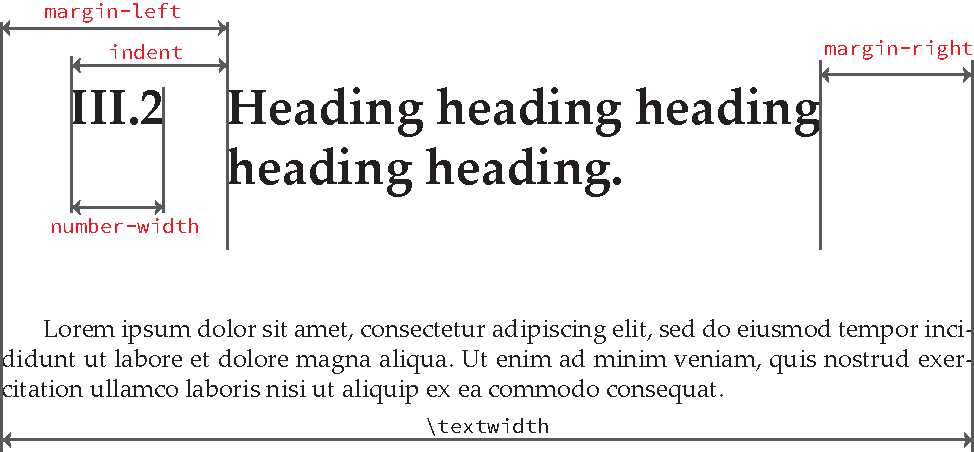
\includegraphics[scale=.7]{images/heading-indent.pdf}}
  \tpCaption{Heading properties for margins and indentation}
  \label{fig:indent}
\end{tpFigure}

If the value of the \lstinline{indent} and \lstinline{margin-left}
Properties is \texttt{auto} or \texttt{auto-global}, then their
respective values are calculated automatically from the
\textit{natural width} of the \lstinline{Number} component. This
always takes the \lstinline{number-format},
\lstinline{heading-format}, and \lstinline{number-sep} properties into
consideration.

\begin{heading}{paragraph}
  \tpTitle{indent: auto-global; margin-left: <any>}
\end{heading}


\begin{tpFigure}[float-pos=t!]
  \tpNumber{Fig. 3}
  \tpFig{\includegraphics[scale=.7,]{images/heading-auto-global.pdf}}
  \tpCaption{\lstinline{indent} set to \lstinline{auto-global} for
    the heading levels~1 through~3. The \lstinline{x-number-width}
    properties represent the respective \textit{maximum number width}
    for each heading level~\lstinline{x}.}
  \label{fig:auto-global}
\end{tpFigure}

If \lstinline{indent} is set to \lstinline{auto-global}, then the
hanging indent of the first line of an item is set to the negative of
the width of the widest \lstinline{Number} across all heading
levels. Values assigned to the \lstinline{margin-left} Property are
discarded. The overall left margin of the rendered item is the width
of the widest number, resulting in a \textit{hanging indent} that is
the same for all headings and exactly the width of the widest
number. \ref{fig:auto-global} illustrates this behaviour.

\begin{heading}{paragraph}
  \tpTitle{indent: auto}
\end{heading}

With \lstinline{indent} set to \lstinline{auto}, the calculated first
line indent is set to the width of the widest number in the same
heading level.

\begin{heading}{paragraph}
  \tpTitle{margin-left: auto}
\end{heading}

With \lstinline{margin-left} set to \lstinline{auto}, the calculated
value for both properties is set to the width of the widest number of
the same heading level \textit{plus} the left margin of the
\textit{preceeding} heading level.

\begin{heading}{paragraph}
  \tpTitle{margin-left: <dimen>}
\end{heading}


If \lstinline{margin-left} is set to a fixed value then this value
will be used as left margin.

\begin{heading}{paragraph}
  \tpTitle{margin-left: <empty>, indent: <auto>}
\end{heading}


If \lstinline{margin-left} is not set but \lstinline{indent} is set to
\lstinline{auto}, then the calculated left margin will be set to the
calculated width of the indent.

\begin{heading}{paragraph}
  \tpTitle{margin-left: <empty>, indent: <empty>}
\end{heading}

If both Properties are unset, no indent or margin will be used at all.


\begin{heading}[label=sec:hdg:toc-indent]{subsection}
  \tpTitle{Indention in the Table of Contents}\index{Indentation!Table of Contents}\index{Margins!Table of Contents}\index{Table of Contents!Indentation}\index{Table of Contents!Margins}
\end{heading}

Indentation in ToC entries works the same as in the actual heading
environments. Simply add \lstinline{toc-} to the left of the property
names to set up the ToC specific behaviour.


\begin{heading}[label=sec:hdg:unnumbered-indent]{subsection}
  \tpTitle{Indention of unnumbered headings}
\end{heading}

Unnumbered headings of a level with indention will be indented as
well, unless you explicitely set the \lstinline{\leftskip} register to
0pt when the \lstinline{Number} or \lstinline{TocNumber} Components
for a heading instance are empty.  You can do that by inserting
\begin{lstlisting}
\tpIfComp{Number}{}{\leftskip=0pt}%
\end{lstlisting}
or
\begin{lstlisting}
\tpIfComp{TocNumber}{}{\leftskip=0pt}%
\end{lstlisting}
respectively at the very top of the overrides for
\lstinline{heading-block} and \lstinline{toc-heading}.

